%iffalse
\let\negmedspace\undefined
\let\negthickspace\undefined
\documentclass[journal,12pt,onecolumn]{exam}
\usepackage[version=4]{mhchem}
\usepackage{chemformula} % for \ch if needed
\usepackage{chemfig}
\usepackage{chemmacros}
\chemsetup{modules = reactions} % Enables reaction arrows
\usepackage{graphicx}
\graphicspath{ {./images/} }

\usepackage{fancyhdr}
\usepackage{geometry}
\usepackage{lastpage}
\usepackage{cite}
\usepackage{amsmath,amssymb,amsfonts,amsthm}
\usepackage{enumitem,multicol}
\usepackage{algorithmic}
\usepackage{graphicx}
\usepackage{textcomp}
\usepackage{xcolor}
\usepackage{txfonts}
\usepackage{listings}
\usepackage{enumitem}
\usepackage{mathtools}
\usepackage{gensymb}
\usepackage{comment}
\usepackage[breaklinks=true]{hyperref}
\usepackage{tkz-euclide} 
\usepackage{listings}
\usepackage{gvv}                                        
%\def\inputGnumericTable{}                                 
\usepackage[latin1]{inputenc}                                
\usepackage{color}                                            
\usepackage{array}                                            
\usepackage{longtable}                                       
\usepackage{calc}                                             
\usepackage{multirow}                                         
\usepackage{hhline}                                           
\usepackage{ifthen}                                           
\usepackage{lscape}
\usepackage{tabularx}
\usepackage{array}
\usepackage{float}

\usepackage{setspace}
\usepackage{lipsum}



\newtheorem{theorem}{Theorem}[section]
\newtheorem{problem}{Problem}
\newtheorem{proposition}{Proposition}[section]
\newtheorem{lemma}{Lemma}[section]
\newtheorem{corollary}[theorem]{Corollary}
\newtheorem{example}{Example}[section]
\newtheorem{definition}[problem]{Definition}
\newcommand{\BEQA}{\begin{eqnarray}}
\newcommand{\EEQA}{\end{eqnarray}}
\newcommand{\define}{\stackrel{\triangle}{=}}
\theoremstyle{remark}

\geometry{margin=1 in}

\pagestyle{fancy}
\fancyhead[L]{2015}
\fancyhead[C]{}
\fancyhead[R]{CY}
\fancyfoot[L]{CY}
\fancyfoot[C]{}
\fancyfoot[R]{\thepage/\pageref{LastPage}}

\setlength{\headheight}{14pt}
\setlength{\headsep}{5pt}
\setlength{\footskip}{20pt}


% Line thickness
\renewcommand{\headrulewidth}{0.4pt}
\renewcommand{\footrulewidth}{0.4pt}



\setlength{\parindent}{0pt} % No paragraph indent

% Define colors and symbols
\definecolor{correctgreen}{rgb}{0,0.5,0}
\definecolor{wrongred}{rgb}{0.8,0,0}

\newcommand{\correct}{\textcolor{correctgreen}{\checkmark}}
\newcommand{\wrong}{\textcolor{wrongred}{\ding{55}}} % X mark, requires amssymb or pifont

% Since amssymb doesn't have ding symbols, let's load pifont for check and cross
\usepackage{pifont}
\newcommand{\cross}{\textcolor{wrongred}{\ding{55}}}
\newcommand{\tick}{\textcolor{correctgreen}{\ding{51}}}


\begin{document}



\title{
ASSIGNMENT 3: GATE 2015 
CY: CHEMISTRY}
\author{AI25BTECH11021 - Abhiram Reddy N}
\maketitle


\begin{center}
    \Large{\textbf{Graduate Aptitude Test In Engineering}}
\end{center}

\textbf{Notations :}

\begin{enumerate}
    \item Options shown in \textcolor{correctgreen}{green} color and with \tick{} icon are correct.
    \item Options shown in \textcolor{wrongred}{red} color and with \cross{} icon are incorrect.
\end{enumerate}

 

\textbf{Question Paper Name:} CY: CHEMISTRY 31st Jan Shift1 
\textbf{Number of Questions:} 65 
\textbf{Total Marks:} 100.0

 

\fbox{\parbox{\linewidth}{
\centering
Wrong answer for MCQ will result in negative marks, (-1/3) for 1 mark Questions and (-2/3) for 2 marks Questions.
}}

 

\begin{center}
\textbf{General Aptitude} \\
Number of Questions: 10 \\
Section Marks: 15.0
\end{center}

 

\fbox{\parbox{\linewidth}{
Q.1 to Q.5 carry 1 mark each \& Q.6 to Q.10 carry 2 marks each.
}}

 
\begin{enumerate}



\item

Choose the most appropriate word from the options given below to complete the following sentence.

The principal presented the chief guest with a \underline{\hspace{4cm}}, as token of appreciation.

\hfill{\brak{\textbf{GATE CY 2015}}}

 

\begin{multicols}{4}
 \begin{enumerate}
    \item \textcolor{wrongred}{\cross\ A momento}
    \item \textcolor{correctgreen}{\tick\ B memento}
    \item \textcolor{wrongred}{\cross\ C momentum}
    \item \textcolor{wrongred}{\cross\ D moment}
\end{enumerate}
\end{multicols}

 

% --- Question 2 ---
\item

Choose the appropriate word/phrase, out of the four options given below, to complete the following sentence:

Frogs \underline{\hspace{4cm}}

\hfill{\brak{\textbf{GATE CY 2015}}}

 

\begin{multicols}{4}
 \begin{enumerate}
    \item \textcolor{correctgreen}{\tick\ A croak}
    \item \textcolor{wrongred}{\cross\ B roar}
    \item \textcolor{wrongred}{\cross\ C hiss}
    \item \textcolor{wrongred}{\cross\ D patter}
\end{enumerate}
\end{multicols}

 

% --- Question 3 ---
\item

% Add question 3 text here
Choose the word most similar to the given word : 
 
Educe

\hfill{\brak{\textbf{GATE CY 2015}}}

 

\begin{multicols}{4}
 \begin{enumerate}
    \item \textcolor{correctgreen}{\tick\ Exert}
    \item \textcolor{wrongred}{\cross\ Educate}
    \item \textcolor{wrongred}{\cross\ Extract}
    \item \textcolor{wrongred}{\cross\ Extend}
\end{enumerate}
\end{multicols}

 


\item

Operators \(\square\), \(\diamond\) and \(\to\) are defined by: 
\(a \square b = \frac{a-b}{a+b}; \quad a \diamond b = \frac{a+b}{a-b}; \quad a \to b = ab.\)

Find the value of \((66 \square 6) \to (66 \diamond 6)\).

 

\hfill{\brak{\textbf{GATE CY 2015}}}

 

\begin{multicols}{4}
 \begin{enumerate}
    \item \textcolor{wrongred}{\cross\ -2}
    \item \textcolor{wrongred}{\cross\ -1}
    \item \textcolor{correctgreen}{\tick\ 1}
    \item \textcolor{wrongred}{\cross\ 2}
\end{enumerate}
\end{multicols}

 

\item

If \(\log_x (5/7) = -1/3\), then the value of \(x\) is

 

\hfill{\brak{\textbf{GATE CY 2015}}}

 

\begin{multicols}{4}
 \begin{enumerate}
    \item \textcolor{correctgreen}{\tick\ 343/125}
    \item \textcolor{wrongred}{\cross\ 125/343}
    \item \textcolor{wrongred}{\cross\ -25/49}
    \item \textcolor{wrongred}{\cross\ -49/25}
\end{enumerate}
\end{multicols}

 

\item

The following question presents a sentence, part of which is underlined. Beneath the sentence you find four ways of phrasing the underlined part. Following the requirements of the standard written English, select the answer that produces the most effective sentence.

 

Tuberculosis, together with its effects, \textbf{ranks one of the leading causes of death} in India.

 

\hfill{\brak{\textbf{GATE CY 2015}}}

 

\begin{multicols}{4}
 \begin{enumerate}
    \item \textcolor{correctgreen}{\tick\ ranks as one of the leading causes of death}
    \item \textcolor{wrongred}{\cross\ rank as one of the leading causes of death}
    \item \textcolor{wrongred}{\cross\ has the rank of one of the leading causes of death}
    \item \textcolor{wrongred}{\cross\ are one of the leading causes of death}
\end{enumerate}
\end{multicols}

 




\item

Read the following paragraph and choose the correct statement.

Climate change has reduced human security and threatened human well being. An ignored reality of human progress is that human security largely depends upon environmental security. But on the contrary, human progress seems contradictory to environmental security. To keep up both at the required level is a challenge to be addressed by one and all. One of the ways to curb the climate change may be suitable scientific innovations, while the other may be the Gandhian perspective on small scale progress with focus on sustainability.

 

\hfill{\brak{\textbf{GATE CY 2015}}}

 

\begin{multicols}{4}
 \begin{enumerate}
    \item \textcolor{wrongred}{\cross\ Human progress and security are positively associated with environmental security.}
    \item \textcolor{correctgreen}{\tick\ Human progress is contradictory to environmental security.}
    \item \textcolor{wrongred}{\cross\ Human security is contradictory to environmental security.}
    \item \textcolor{wrongred}{\cross\ Human progress depends upon environmental security.}
\end{enumerate}
\end{multicols}

 

\item

Fill in the missing value

 

\begin{figure}
    \centering
    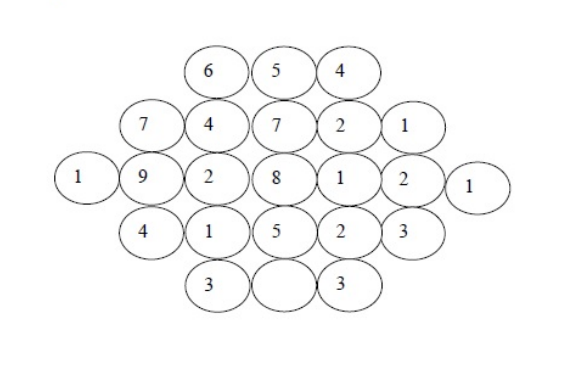
\includegraphics[width=\textwidth]{figs/image1.png}
    \caption{}
    \label{fig:figure1}
\end{figure}

 

Correct Answer : \textcolor{correctgreen}{3}

 

\item

A cube of side 3 units is formed using a set of smaller cubes of side 1 unit. Find the proportion of the number of faces of the smaller cubes visible to those which are NOT visible.

 

\hfill{\brak{\textbf{GATE CY 2015}}}

 

\begin{multicols}{4}
 \begin{enumerate}
    \item \textcolor{wrongred}{\cross\ 1 : 4}
    \item \textcolor{wrongred}{\cross\ 1 : 3}
    \item \textcolor{correctgreen}{\tick\ 1 : 2}
    \item \textcolor{wrongred}{\cross\ 2 : 3}
\end{enumerate}
\end{multicols}

 

\item 

Humpty Dumpty sits on a wall every day while having lunch. The wall sometimes breaks. A person sitting on the wall falls if the wall breaks.

Which one of the statements below is logically valid and can be inferred from the above sentences?

\hfill{\brak{\textbf{GATE CY 2015}}}

 

\begin{multicols}{2}
\begin{enumerate}
    \item \textcolor{red}{\wrong} A) Humpty Dumpty always falls while having lunch
    \item \textcolor{green}{\correct} B) Humpty Dumpty does not fall sometimes while having lunch
    \item \textcolor{red}{\wrong} C) Humpty Dumpty never falls during dinner
    \item \textcolor{red}{\wrong} D) When Humpty Dumpty does not sit on the wall, the wall does not break
\end{enumerate}
\end{multicols}
 



\begin{center}
\textbf{Chemistry} \\
Number of Questions: \hspace{3 cm} 55 \\
Section Marks: \hspace{4 cm} 85.0
\end{center}

 

\noindent\framebox{\parbox{\linewidth}{
\textbf{Q.11 to Q.35 carry 1 mark each \& Q.36 to Q.65 carry 2 marks each.}
}}

 

% Question 11

\item 

Which one of the following plots represents an acceptable wavefunction?

\begin{center}
\begin{tikzpicture}[scale=1.2]

% Plot A
\begin{scope}[shift={(0,0)}]
\draw[->] (0,0) -- (2,0) node[right] {$x$};
\draw[->] (0,0) -- (0,2) node[above] {$\Psi$};
\draw[thick] plot[smooth, tension=0.7] coordinates {(0,0.5) (0.5,1.5) (1,1.3) (1.5,1.8) (2,1.6)};
\node at (1,-0.4) {(A)};
\end{scope}

% Plot B
\begin{scope}[shift={(3.5,0)}]
\draw[->] (0,0) -- (2,0) node[right] {$x$};
\draw[->] (0,0) -- (0,2) node[above] {$\Psi$};
\draw[thick] plot[variable=\t, domain=0:2, samples=100] 
    ({\t}, {0.5 + 0.4*sin(3.14*\t*2)});
\node at (1,-0.4) {(B)};
\end{scope}

% Plot C
\begin{scope}[shift={(0,-3)}]
\draw[->] (0,0) -- (2,0) node[right] {$x$};
\draw[->] (0,0) -- (0,2) node[above] {$\Psi$};
\draw[thick] (0,0) -- (1,2) -- (2,0);
\node at (1,-0.4) {(C)};
\end{scope}

% Plot D
\begin{scope}[shift={(3.5,-3)}]
\draw[->] (0,0) -- (2,0) node[right] {$x$};
\draw[->] (0,0) -- (0,2) node[above] {$\Psi$};
\draw[thick] plot[variable=\t, domain=0:2, samples=100] 
    ({\t}, {0.5 + 0.4*sin(3.14*\t*6)});
\node at (1,-0.4) {(D)};
\end{scope}

\end{tikzpicture}
\end{center}

\hfill{\brak{\textbf{GATE CY 2015}}}

 

\begin{multicols}{2}
\begin{enumerate}
    \item \textcolor{red}{\wrong} A
    \item \textcolor{red}{\wrong} B
    \item \textcolor{red}{\wrong} C
    \item \textcolor{green}{\correct} D
\end{enumerate}
\end{multicols}

 



\item 

When the operator, $-\hbar^{2} \frac{d^2}{dx^2}$, operates on the function $e^{-ikx}$, the result is

\hfill{\brak{\textbf{GATE CY 2015}}}

 

\begin{multicols}{2}
\begin{enumerate}
    \item \textcolor{green}{\correct} $(A) \quad \hbar^2 k^2 e^{-ikx}$
    \item \textcolor{red}{\wrong} $(B) \quad ik \hbar^2 e^{-ikx}$
    \item \textcolor{red}{\wrong} $(C) \quad \hbar^2 e^{-ikx}$
    \item \textcolor{red}{\wrong} $(D) \quad \hbar^2 e^{-ikx}$
\end{enumerate}
\end{multicols}

 


\item 

\begin{figure}
    \centering
    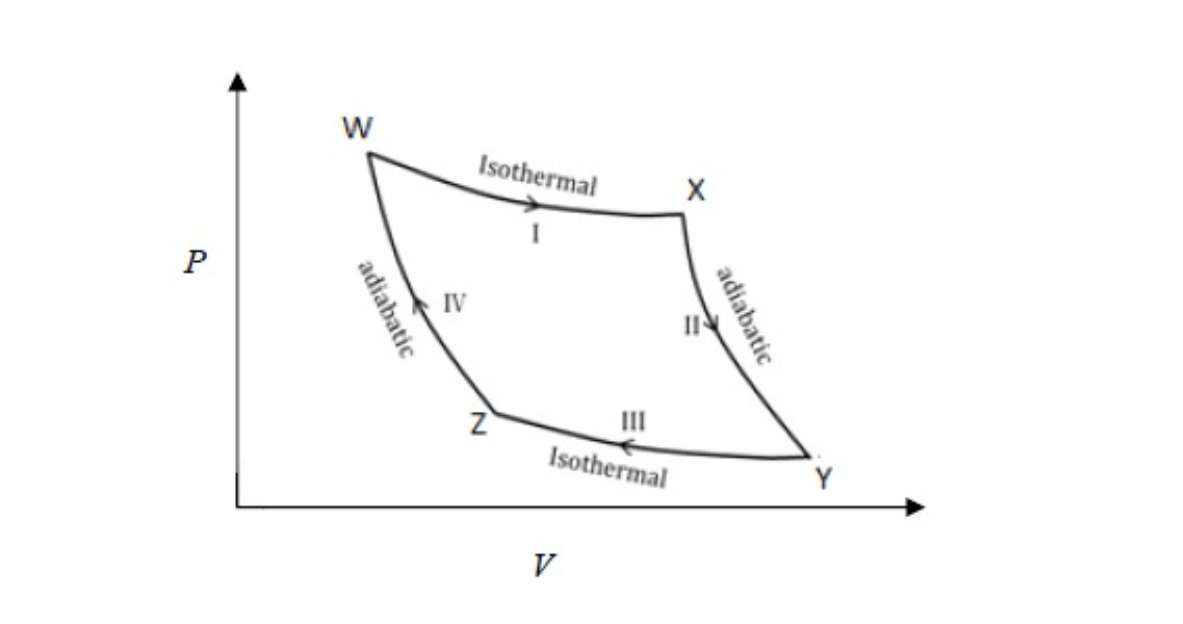
\includegraphics[width=\textwidth]{figs/image2.png}
    \caption{}
    \label{fig:figure2}
\end{figure}

From the above Carnot cycle undergone by an ideal gas, identify the processes in which the change in internal energy is \textbf{NON-ZERO}.

\hfill{\brak{\textbf{GATE CY 2015}}}

 

\begin{multicols}{2}
\begin{enumerate}
    \item \textcolor{red}{\ding{55}} I and II
    \item \textcolor{green}{\checkmark} II and IV
    \item \textcolor{red}{\ding{55}} II and III
    \item \textcolor{red}{\ding{55}} I and IV
\end{enumerate}
\end{multicols}

 

% Question 14
\item 

For an ideal gas with molar mass $M$, the molar translational entropy at a given temperature is proportional to

\hfill{\brak{\textbf{GATE CY 2015}}}

 

\begin{multicols}{2}
\begin{enumerate}
    \item \textcolor{red}{\ding{55}} $M^{3/2}$
    \item \textcolor{red}{\ding{55}} $M^{1/2}$
    \item \textcolor{red}{\ding{55}} $e^M$
    \item \textcolor{green}{\checkmark} $\ln(M)$
\end{enumerate}
\end{multicols}

 

% Question 15
\item 

Which one of the following defines the absolute temperature of a system?

\hfill{\brak{\textbf{GATE CY 2015}}}

 

\begin{multicols}{2}
\begin{enumerate}
    \item \textcolor{green}{\checkmark} $\left(\frac{\partial U}{\partial S}\right)_V$
    \item \textcolor{red}{\ding{55}} $\left(\frac{\partial A}{\partial S}\right)_V$
    \item \textcolor{red}{\ding{55}} $\left(\frac{\partial H}{\partial S}\right)_V$
    \item \textcolor{red}{\ding{55}} $\left(\frac{\partial G}{\partial S}\right)_V$
\end{enumerate}
\end{multicols}

 



% Question 16
\item 
Which of the following properties are characteristic of an ideal solution?

\begin{enumerate}
    \item[(i)] $\Delta_\text{mix} G_{T,P}$ is negative
    \item[(ii)] $\Delta_\text{mix} S_{T,P}$ is positive
    \item[(iii)] $\Delta_\text{mix} V_{T,P}$ is positive
    \item[(iv)] $\Delta_\text{mix} H_{T,P}$ is negative
\end{enumerate}

(A) (i) and (iv) \quad (B) (i) and (ii) \quad (C) (i) and (iii) \quad (D) (iii) and (iv)

\hfill{\brak{\textbf{GATE CY 2015}}}

 

\begin{multicols}{2}
\begin{enumerate}
    \item \textcolor{red}{\ding{55}} A
    \item \textcolor{green}{\checkmark} B
    \item \textcolor{red}{\ding{55}} C
    \item \textcolor{red}{\ding{55}} D
\end{enumerate}
\end{multicols}

 

% Question 17
\item 
The expression for the equilibrium constant ($K_{eq}$) for the enzyme-catalyzed reaction is given below.

\begin{center}
\begin{tikzpicture}[scale=1.1, every node/.style={font=\normalsize}]
  % Nodes
  \node (E) at (0,0) {E + S};
  \node (ES) at (3,0) {ES};
  \node (P) at (6,0) {P + E};

  % Arrows
  \draw[->] (E) -- node[above] {$k_1$} (ES);
  \draw[<-] (E) -- node[below] {$k_2$} (ES);

  \draw[->] (ES) -- node[above] {$k_3$} (P);
  \draw[<-] (ES) -- node[below] {$k_4$} (P);
\end{tikzpicture}
\end{center}

\hfill{\brak{\textbf{GATE CY 2015}}}

 

\begin{multicols}{2}
\begin{enumerate}
    \item \textcolor{green}{\checkmark} $\dfrac{k_1 k_3}{k_2 k_4}$
    \item \textcolor{red}{\ding{55}} $\dfrac{k_1 k_2}{k_3 k_4}$
    \item \textcolor{red}{\ding{55}} $\dfrac{k_3 k_2}{k_1 k_4}$
    \item \textcolor{red}{\ding{55}} $\dfrac{k_1 k_4}{k_2 k_3}$
\end{enumerate}
\end{multicols}

 

% Question 18
\item 

Given the $E^0$ values for the following reaction sequence,
\[
\text{Mn}^{6+} \xrightarrow{1.28\text{ V}} \text{Mn}^{5+} \xrightarrow{2.9\text{ V}} \text{Mn}^{4+} \xrightarrow{0.96\text{ V}} \text{Mn}^{3+} \xrightarrow{1.5\text{ V}} \text{Mn}^{2+}
\]
The computed value of $E^0$ for Mn$^{6+} \rightarrow$ Mn$^{2+}$ (in volts) is \underline{\hspace{3cm}}

\hfill{\brak{\textbf{GATE CY 2015}}}
 

\textbf{Correct answer:} \\
\textcolor{green}{1.6 to 1.7}

 

%----------------- Q19 ------------------
\item 
The absorption spectrum of [Ti(H$_2$O)$_6$]$^{3+}$ in solution comprises of a maximum with a shoulder. The reason for the shoulder is

\begin{enumerate}
    \item ligand-to-metal charge transfer (LMCT)
    \item metal-to-ligand charge transfer (MLCT)
    \item Jahn-Teller distortion
    \item nephelauxetic effect
\end{enumerate}

\hfill{\brak{\textbf{GATE CY 2015}}}

 

\begin{multicols}{2}
\begin{enumerate}
    \item \wrong A
    \item \wrong B
    \item \correct C
    \item \wrong D
\end{enumerate}
\end{multicols}

 

%----------------- Q20 ------------------
\item 
The ease of formation of the adduct, NH$_3\cdot$BX$_3$ (where, X = F, Cl, Br) follows the order

\begin{enumerate}
    \item BBr$_3$ < BCl$_3$ < BF$_3$
    \item BCl$_3$ < BF$_3$ < BBr$_3$
    \item BF$_3$ < BCl$_3$ < BBr$_3$
    \item BBr$_3$ < BF$_3$ < BCl$_3$
\end{enumerate}

\hfill{\brak{\textbf{GATE CY 2015}}}

 

\begin{multicols}{2}
\begin{enumerate}
    \item \wrong A
    \item \wrong B
    \item \correct C
    \item \wrong D
\end{enumerate}
\end{multicols}

 

%----------------- Q21 ------------------
\item 
An efficient catalyst for hydrogenation of alkenes is [Rh(PPh$_3$)$_3$Cl]. However, [Ir(PPh$_3$)$_3$Cl] does not catalyze this reaction, because

\begin{enumerate}
    \item PPh$_3$ binds stronger to Ir than to Rh
    \item Cl binds stronger to Ir than to Rh
    \item PPh$_3$ binds stronger to Rh than to Ir
    \item Cl binds stronger to Rh than to Ir
\end{enumerate}

\hfill{\brak{\textbf{GATE CY 2015}}}

 

\begin{multicols}{2}
\begin{enumerate}
    \item \correct A
    \item \wrong B
    \item \wrong C
    \item \wrong D
\end{enumerate}
\end{multicols}

 

%----------------- Q22 ------------------
\item 
Among the given pH values, the O$_2$ binding efficiency of heamoglobin is maximum at

\begin{enumerate}
    \item 6.8
    \item 7.0
    \item 7.2
    \item 7.4
\end{enumerate}

\hfill{\brak{\textbf{GATE CY 2015}}}

 

\begin{multicols}{2}
\begin{enumerate}
    \item \wrong A
    \item \wrong B
    \item \wrong C
    \item \correct D
\end{enumerate}
\end{multicols}



%----------------- Q23 ------------------
\item 
The intense red color of [Fe(bpy)$_3$]$^{2+}$ (bpy = 2,2'-bipyridine) is due to

\begin{enumerate}
    \item metal-to-ligand charge transfer (MLCT)
    \item ligand-to-metal charge transfer (LMCT)
    \item d-d transition
    \item inter-valence charge transfer (IVCT)
\end{enumerate}

\hfill{\brak{\textbf{GATE CY 2015}}}

 

\begin{multicols}{2}
\begin{enumerate}
    \item \correct A
    \item \wrong B
    \item \wrong C
    \item \wrong D
\end{enumerate}
\end{multicols}

 

%----------------- Q24 ------------------
\item 
The compound with planar geometry is

\begin{enumerate}
    \item N(t-Bu)$_3$
    \item NPh$_3$
    \item NF$_3$
    \item N(SiH$_3$)$_3$
\end{enumerate}

\hfill{\brak{\textbf{GATE CY 2015}}}

 

\begin{multicols}{2}
\begin{enumerate}
    \item \wrong A
    \item \wrong B
    \item \wrong C
    \item \correct D
\end{enumerate}
\end{multicols}

 

%----------------- Q25 ------------------
\item 
The electrical conductivity of a metal

\begin{enumerate}
    \item increases with increasing temperature
    \item decreases with increasing temperature
    \item is independent of temperature
    \item shows oscillatory behaviour with temperature
\end{enumerate}

\hfill{\brak{\textbf{GATE CY 2015}}}

 

\begin{multicols}{2}
\begin{enumerate}
    \item \wrong A
    \item \correct B
    \item \wrong C
    \item \wrong D
\end{enumerate}
\end{multicols}

 

%----------------- Q26 ------------------
\item 
Which one of the following statements is \textbf{INCORRECT}?

\begin{enumerate}
    \item Frenkel defect is a cation vacancy and a cation interstitial.
    \item Frenkel defect is an anion vacancy and a cation interstitial.
    \item Density of a solid remains unchanged in case of Frenkel defects.
    \item Density of a solid decreases in case of Schottky defects.
\end{enumerate}

\hfill{\brak{\textbf{GATE CY 2015}}}

 

\begin{multicols}{2}
\begin{enumerate}
    \item \wrong A
    \item \correct B
    \item \wrong C
    \item \wrong D
\end{enumerate}
\end{multicols}

 


%----------------- Q27 ------------------
\item 
The absolute configuration of C2 and C3 in the following compound is

\begin{figure}[H]
    \centering
    
\includegraphics[width=0.3\textwidth]{figs/image3.png} 
    \caption{}
    \label{fig:figure3}
    
    % Replace with actual image filename
\end{figure}

\begin{enumerate}
    \item $2R, 3S$
    \item $2S, 3R$
    \item $2S, 3S$
    \item $2R, 3R$
\end{enumerate}

\hfill{\brak{\textbf{GATE CY 2015}}}

\begin{multicols}{2}
\begin{enumerate}
    \item \wrong A
    \item \wrong B
    \item \wrong C
    \item \correct D
\end{enumerate}
\end{multicols}


%----------------- Q28 ------------------
\item 
Among the following compounds, the one that is non-aromatic, is

\begin{figure}[H]
    \centering
    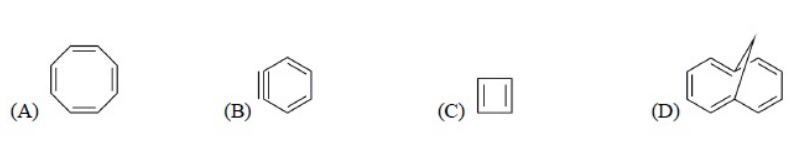
\includegraphics[width=0.5\textwidth]{figs/image4.png} 
    \caption{}
    \label{fig:figure4}
    
    % Replace with actual image filename
\end{figure}

\begin{enumerate}
    \item A
    \item B
    \item C
    \item D
\end{enumerate}

\hfill{\brak{\textbf{GATE CY 2015}}}

\begin{multicols}{2}
\begin{enumerate}
    \item \correct A
    \item \wrong B
    \item \wrong C
    \item \wrong D
\end{enumerate}
\end{multicols}


%----------------- Q29 ------------------
\item 
The correct order of reactivity of \emph{p}-halonitrobenzenes in the following reaction is

\begin{figure}[H]
    \centering
    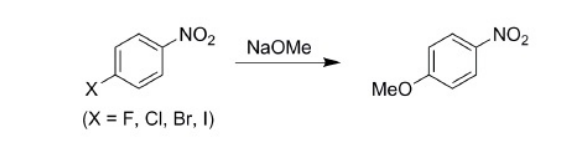
\includegraphics[width=0.6\textwidth]{figs/image5.png}
    \caption{}
    \label{fig:figure5}
    
    % Replace with actual image filename
\end{figure}

\begin{enumerate}
    \item p-chloronitrobenzene $>$ p-iodonitrobenzene $>$ p-fluoronitrobenzene $>$ p-bromonitrobenzene
    \item p-fluoronitrobenzene $>$ p-chloronitrobenzene $>$ p-bromonitrobenzene $>$ p-iodonitrobenzene
    \item p-iodonitrobenzene $>$ p-bromonitrobenzene $>$ p-chloronitrobenzene $>$ p-fluoronitrobenzene
    \item p-bromonitrobenzene $>$ p-fluoronitrobenzene $>$ p-iodonitrobenzene $>$ p-chloronitrobenzene
\end{enumerate}

\hfill{\brak{\textbf{GATE CY 2015}}}

\begin{multicols}{2}
\begin{enumerate}
    \item \correct A
    \item \wrong B
    \item \wrong C
    \item \wrong D
\end{enumerate}
\end{multicols}





%----------------- Q30 ------------------
\item 
Tollen's test is \textbf{NEGATIVE} for

\begin{enumerate}
    \item mannose
    \item maltose
    \item glucose
    \item sucrose
\end{enumerate}

\hfill{\brak{\textbf{GATE CY 2015}}}

\begin{multicols}{2}
\begin{enumerate}
    \item \wrong A
    \item \wrong B
    \item \wrong C
    \item \correct D
\end{enumerate}
\end{multicols}


%----------------- Q31 ------------------
\item 
The compound given below is a

\begin{figure}[H]
    \centering
    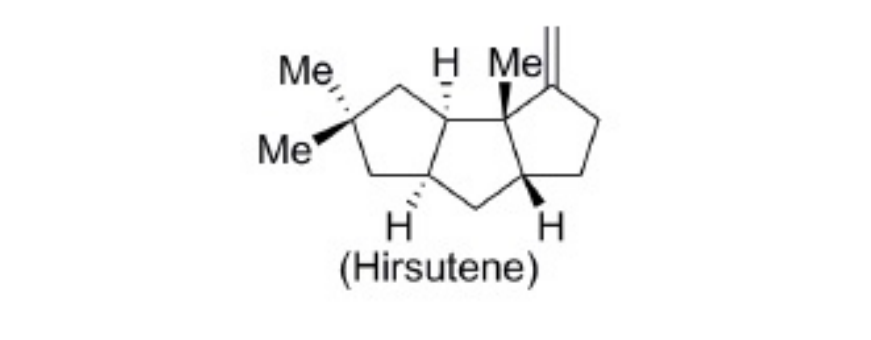
\includegraphics[width=0.35\textwidth]{figs/image6.png} % Replace with actual image filename
    \caption{Structure of Hirsutene}
    \label{fig:hirsutene}
\end{figure}

\begin{enumerate}
    \item sesterterpene
    \item monoterpene
    \item sesquiterpene
    \item triterpene
\end{enumerate}

\hfill{\brak{\textbf{GATE CY 2015}}}

\begin{multicols}{2}
\begin{enumerate}
    \item \wrong A
    \item \wrong B
    \item \correct C
    \item \wrong D
\end{enumerate}
\end{multicols}


%----------------- Q32 ------------------
\item 
Amongst the following, the compound that \textbf{DOES NOT} act as a diene in Diels-Alder reaction is

\begin{figure}[H]
    \centering
    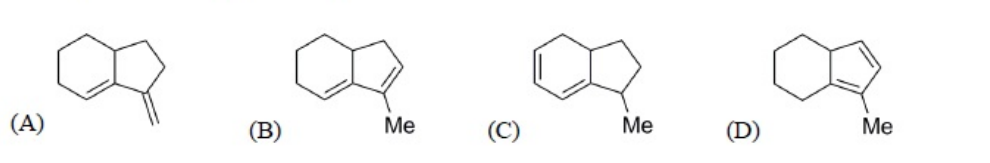
\includegraphics[width=0.6\textwidth]{figs/image7.png} % Replace with actual image filename
    \caption{Options for Diels–Alder reaction diene}
    \label{fig:diels_alder_diene}
\end{figure}

\begin{enumerate}
    \item A
    \item B
    \item C
    \item D
\end{enumerate}

\hfill{\brak{\textbf{GATE CY 2015}}}

\begin{multicols}{2}
\begin{enumerate}
    \item \wrong A
    \item \wrong B
    \item \correct C
    \item \wrong D
\end{enumerate}
\end{multicols}




%----------------- Q33 ------------------
\item 
The following conversion is an example of

\begin{figure}[H]
    \centering
    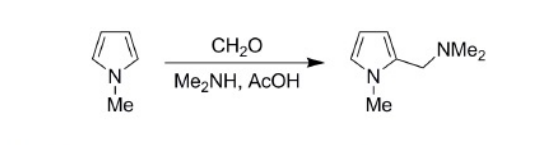
\includegraphics[width=0.45\textwidth]{figs/image8.png} % Replace with actual image filename
    \caption{Reaction conversion involving hydrazone and Me$_2$NH}
    \label{fig:conversion33}
\end{figure}

\begin{enumerate}
    \item Arndt-Eistert homologation
    \item Mannich reaction
    \item Michael addition
    \item Chichibabin amination reaction
\end{enumerate}

\hfill{\brak{\textbf{GATE CY 2015}}}

\begin{multicols}{2}
\begin{enumerate}
    \item \correct A
    \item \wrong B
    \item \wrong C
    \item \wrong D
\end{enumerate}
\end{multicols}


%----------------- Q34 ------------------
\item 
The mass spectrum of a dihalo compound shows peaks with relative intensities of 1:2:1 corresponding to M, M+2 and M+4 (M is the mass of the molecular ion), respectively. The compound is

\begin{figure}[H]
    \centering
    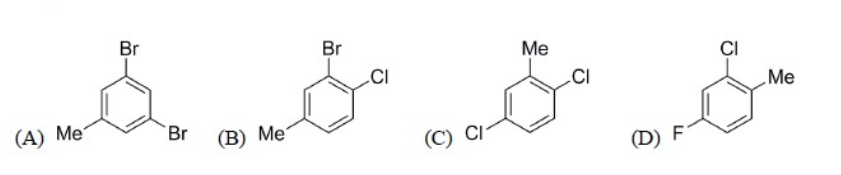
\includegraphics[width=0.6\textwidth]{figs/image9.png} % Replace with actual image filename
    \caption{Structures of dihalo compounds}
    \label{fig:massspectrum34}
\end{figure}

\begin{enumerate}
    \item A
    \item B
    \item C
    \item D
\end{enumerate}

\hfill{\brak{\textbf{GATE CY 2015}}}

\begin{multicols}{2}
\begin{enumerate}
    \item \correct A
    \item \wrong B
    \item \wrong C
    \item \wrong D
\end{enumerate}
\end{multicols}


%----------------- Q35 ------------------
\item 
Reaction of benzaldehyde and \emph{p}-methylbenzaldehyde under McMurry coupling conditions (TiCl$_4$ and LiAlH$_4$) gives a mixture of alkenes. The number of alkenes formed is \underline{\hspace{3cm}}.

\hfill{\brak{\textbf{GATE CY 2015}}}


\textbf{Correct Answer :} \textcolor{green}{6}


%----------------- Q36 ------------------
\item 
The difference in the ground state energies (kJ/mol) of an electron in one-dimensional boxes of lengths 0.2 nm and 2 nm is \underline{\hspace{3cm}}.

\hfill{\brak{\textbf{GATE CY 2015}}}


\textbf{Correct Answer :} \textcolor{green}{880 to 900}







%----------------- Q37 ------------------
\item 
The mean ionic activity coefficient of 0.001 molal ZnSO$_4$ (aq) at 298 K according to the Debye-Huckel limiting law is (Debye-Huckel constant is 0.509 mol$^{-1/2}$) \underline{\hspace{3cm}}

\hfill{\brak{\textbf{GATE CY 2015}}}


\textbf{Correct Answer :} \textcolor{green!60!black}{0.73 to 0.75}


%----------------- Q38 ------------------
\item 
The process given below follows the Langmuir adsorption isotherm.

\begin{figure}[H]
    \centering
    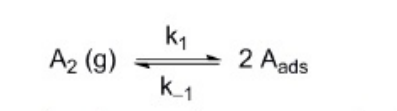
\includegraphics[width=0.4\textwidth]{figs/image10.png} % Replace with actual image filename
    \caption{Langmuir adsorption equilibrium for A$_2$(g) on surface}
    \label{fig:langmuir_adsorption}
\end{figure}

If $\theta$ denotes the surface coverage and $P$ denotes the pressure, the slope of the plot of $1/\theta$ versus $1/P$ is

\begin{enumerate}
    \item $1/(K_{eq})^2$
    \item $1/K_{eq}$
    \item $-1/K_{eq}$
    \item $1/(K_{eq})^{1/2}$
\end{enumerate}

\hfill{\brak{\textbf{GATE CY 2015}}}

\begin{multicols}{2}
\begin{enumerate}
    \item \wrong A
    \item \wrong B
    \item \wrong C
    \item \correct D
\end{enumerate}
\end{multicols}


%----------------- Q39 ------------------
\item 
For a gas phase unimolecular reaction at temperature 298 K, with a pre-exponential factor of $2.17 \times 10^{13}$ s$^{-1}$, the entropy of activation (J K$^{-1}$ mol$^{-1}$) is \underline{\hspace{3cm}}

\hfill{\brak{\textbf{GATE CY 2015}}}


\textbf{Correct Answer :} \textcolor{green!60!black}{102 to 106}


%----------------- Q40 ------------------
\item 
A liquid has vapor pressure of $2.02 \times 10^3$ N m$^{-2}$ at 293 K and heat of vaporization of 41 kJ mol$^{-1}$. The boiling point of the liquid (in Kelvin) is \underline{\hspace{3cm}}

\hfill{\brak{\textbf{GATE CY 2015}}}


\textbf{Correct Answer :} \textcolor{green!60!black}{380 to 385}







%----------------- Q41 ------------------
\item 
The rotational partition function of a diatomic molecule with energy levels corresponding to $J = 0$ and $1$, is (where $\varepsilon$ is a constant)

\begin{enumerate}
    \item $1 + 2e^{-\varepsilon}$
    \item $1 + 3e^{-3\varepsilon}$
    \item $1 + e^{-3\varepsilon}$
    \item $1 + 3e^{-\varepsilon}$
\end{enumerate}

\hfill{\brak{\textbf{GATE CY 2015}}}

\begin{multicols}{2}
\begin{enumerate}
    \item \wrong A
    \item \wrong B
    \item \wrong C
    \item \correct D
\end{enumerate}
\end{multicols}


%----------------- Q42 ------------------
\item 
The internal energy of an ideal gas follows the equation $U = 3.5 \, PV + k$, where $k$ is a constant. The gas expands from an initial volume of 0.25 m$^3$ to a final volume of 0.86 m$^3$. If the initial pressure is 5 N m$^{-2}$, the change in internal energy (in Joules) is (given $PV^{1.3} = \text{constant}$) \underline{\hspace{3cm}}

\hfill{\brak{\textbf{GATE CY 2015}}}

\textbf{Correct Answer :} \textcolor{green!60!black}{-1.38 to -1.33}


%----------------- Q43 ------------------
\item 
The solubility product of AgBr(s) is $5 \times 10^{-13}$ at 298 K. If the standard reduction potential of the half-cell, $E^\circ_{\text{Ag}^+|\text{AgBr}(s)|\text{Br}^-}$ is 0.07 V, the standard reduction potential, $E^\circ_{\text{Ag}^+|\text{Ag}}$ (in volts) is \underline{\hspace{3cm}}

\hfill{\brak{\textbf{GATE CY 2015}}}

\textbf{Correct Answer :} \textcolor{green!60!black}{0.79 to 0.82}


%----------------- Q44 ------------------
\item 
One mole of a substance is heated from 300 K to 400 K at constant pressure. The $C_P$ of the substance is given by, $C_P$ (J K$^{-1}$mol$^{-1}$) = $5 + 0.1\,T$. The change in entropy, in J K$^{-1}$mol$^{-1}$, of the substance is \underline{\hspace{3cm}}

\hfill{\brak{\textbf{GATE CY 2015}}}

\textbf{Correct Answer :} \textcolor{green!60!black}{11.3 to 11.5}




%----------------- Q45 ------------------
\item 
The potential energy (PE) versus reaction coordinate diagrams for electron transfer reactions with rate constants $k_1$, $k_2$, and $k_3$ are given below. The increasing order of the rate constants is

\begin{figure}[H]
    \centering
    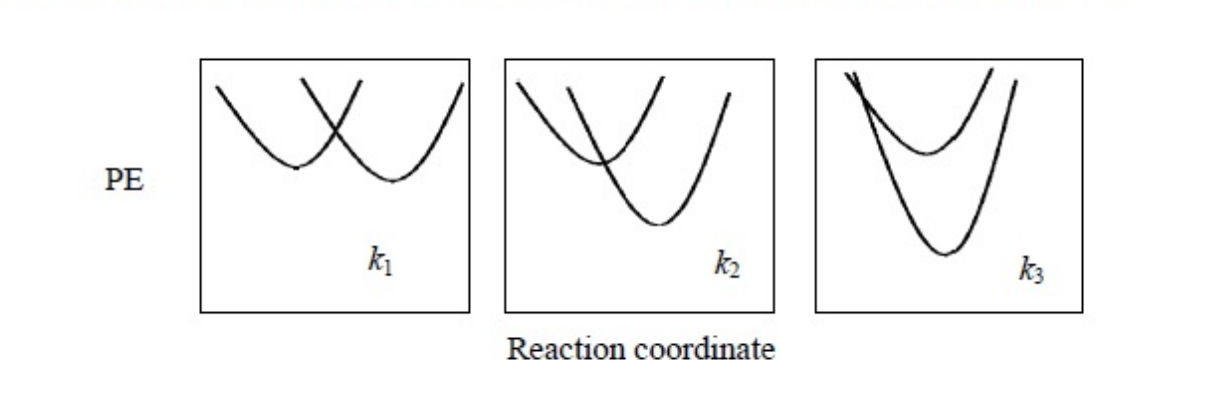
\includegraphics[width=0.5\textwidth]{figs/image11.png} % replace with actual file if used
    \caption{Potential energy diagrams for reactions with rate constants $k_1$, $k_2$, and $k_3$}
    \label{fig:rate_constants}
\end{figure}

\begin{enumerate}
    \item $k_3 < k_2 < k_1$
    \item $k_2 < k_1 < k_3$
    \item $k_1 < k_3 < k_2$
    \item $k_3 < k_1 < k_2$
\end{enumerate}

\hfill{\brak{\textbf{GATE CY 2015}}}

\begin{multicols}{2}
\begin{enumerate}
    \item \wrong A
    \item \wrong B
    \item \wrong C
    \item \correct D
\end{enumerate}
\end{multicols}


%----------------- Q46 ------------------
\item 
The distance between two successive (110) planes in a simple cubic lattice with lattice parameter $a$ is

\begin{enumerate}
    \item $\sqrt{2}\,a$
    \item $\sqrt{3}\,a$
    \item $2\sqrt{2}\,a$
    \item $\dfrac{a}{\sqrt{2}}$
\end{enumerate}

\hfill{\brak{\textbf{GATE CY 2015}}}

\begin{multicols}{2}
\begin{enumerate}
    \item \wrong A
    \item \wrong B
    \item \wrong C
    \item \correct D
\end{enumerate}
\end{multicols}


%----------------- Q47 ------------------
\item 
The percent transmittance of $8 \times 10^{-5}$ M solution of KMnO$_4$ is 39.8 when measured at 510 nm in a cell of path length of 1 cm. The absorbance and the molar extinction coefficient (in M$^{-1}$ cm$^{-1}$) of this solution are, respectively

\begin{enumerate}
    \item 0.30 and 4500
    \item 0.35 and 4800
    \item 0.4 and 5000
    \item 0.48 and 5200
\end{enumerate}

\hfill{\brak{\textbf{GATE CY 2015}}}

\begin{multicols}{2}
\begin{enumerate}
    \item \wrong A
    \item \wrong B
    \item \wrong C
    \item \correct D
\end{enumerate}
\end{multicols}




%----------------- Q48 ------------------
\item 
The value of ‘$g$’ and the number of signals observed for the reference standard, diphenylpicrylhydrazyl (DPPH), in the solid state ESR spectrum are, respectively,

\begin{enumerate}
    \item 2.0036 and 1
    \item 2.0036 and 3
    \item 2.2416 and 1
    \item 2.2416 and 3
\end{enumerate}

\hfill{\brak{\textbf{GATE CY 2015}}}

\begin{multicols}{2}
\begin{enumerate}[leftmargin=*, align=left]
    \item \correct A
    \item \wrong B
    \item \wrong C
    \item \wrong D
\end{enumerate}
\end{multicols}


%----------------- Q49 ------------------
\item 
Ammonolysis of S$_2$Cl$_2$ in an inert solvent gives

\begin{enumerate}
    \item S$_2$N$_2$
    \item S$_2$N$_2$Cl$_2$
    \item S$_2$N$_2$H$_4$
    \item S$_4$N$_4$
\end{enumerate}

\hfill{\brak{\textbf{GATE CY 2015}}}

\begin{multicols}{2}
\begin{enumerate}[leftmargin=*, align=left]
    \item \wrong A
    \item \wrong B
    \item \wrong C
    \item \correct D
\end{enumerate}
\end{multicols}


%----------------- Q50 ------------------
\item 
The complexes K$_2$[NiF$_6$] and K$_3$[CoF$_6$] are

\begin{enumerate}
    \item both paramagnetic
    \item both diamagnetic
    \item paramagnetic and diamagnetic, respectively
    \item diamagnetic and paramagnetic, respectively
\end{enumerate}

\hfill{\brak{\textbf{GATE CY 2015}}}

\begin{multicols}{2}
\begin{enumerate}[leftmargin=*, align=left]
    \item \wrong A
    \item \wrong B
    \item \wrong C
    \item \correct D
\end{enumerate}
\end{multicols}


%----------------- Q51 ------------------
\item 
The point group of IF$_7$ is

\begin{enumerate}
    \item D$_{6h}$
    \item D$_{5h}$
    \item C$_{6v}$
    \item C$_{5v}$
\end{enumerate}

\hfill{\brak{\textbf{GATE CY 2015}}}

\begin{multicols}{2}
\begin{enumerate}[leftmargin=*, align=left]
    \item \wrong A
    \item \correct B
    \item \wrong C
    \item \wrong D
\end{enumerate}
\end{multicols}






%----------------- Q52 ------------------
\item 
When one CO group is replaced by PPh$_3$ in [Cr(CO)$_6$], which one of the following statements is \textbf{TRUE}?

\begin{enumerate}
    \item The Cr-C bond length increases and CO bond length decreases
    \item The Cr-C bond length decreases and CO bond length decreases
    \item The Cr-C bond length decreases and CO bond length increases
    \item The Cr-C bond length increases and CO bond length increases
\end{enumerate}

\hfill{\brak{\textbf{GATE CY 2015}}}

\begin{multicols}{2}
\begin{enumerate}[leftmargin=*, align=left]
    \item \wrong A
    \item \correct B
    \item \wrong C
    \item \wrong D
\end{enumerate}
\end{multicols}


%----------------- Q53 ------------------
\item 
Identify X in the reaction, [Pt(NH$_3$)$_4$]$^{2+}$ + 2 HCl $\rightarrow$ X

\begin{enumerate}
    \item cis-[PtCl$_2$(NH$_3$)$_2$]
    \item trans-[PtCl$_2$(NH$_3$)$_2$]
    \item [PtCl(NH$_3$)]$^+$
    \item [PtCl$_2$(NH$_3$)]$^+$
\end{enumerate}

\hfill{\brak{\textbf{GATE CY 2015}}}

\begin{multicols}{2}
\begin{enumerate}[leftmargin=*, align=left]
    \item \correct A
    \item \wrong B
    \item \wrong C
    \item \wrong D
\end{enumerate}
\end{multicols}


%----------------- Q54 ------------------
\item 
Identify the function of hemocyanin and the metal responsible for it.

\begin{enumerate}
    \item O$_2$ transport and Fe
    \item O$_2$ transport and Cu
    \item electron transport and Fe
    \item electron transport and Cu
\end{enumerate}

\hfill{\brak{\textbf{GATE CY 2015}}}

\begin{multicols}{2}
\begin{enumerate}[leftmargin=*, align=left]
    \item \wrong A
    \item \correct B
    \item \wrong C
    \item \wrong D
\end{enumerate}
\end{multicols}


%----------------- Q55 ------------------
\item 
The limiting current (in $\mu$A) from the reduction of $3 \times 10^{-4}$ M Pb$^{2+}$ using a dropping mercury electrode (DME) with characteristics, $m = 3.0$ mg s$^{-1}$ and $t = 3$ s, is \\
(diffusion coefficient of Pb$^{2+}$ = $1.2 \times 10^{-5}$ cm$^2$ s$^{-1}$)

\hfill{\brak{\textbf{GATE CY 2015}}}

\textcolor{green}{\textbf{Correct Answer :}} 3.5 to 3.8







%----------------- Q56 ------------------
\item 
The number of possible stereoisomers obtained in the following reaction is 
\begin{figure}[H]
\centering
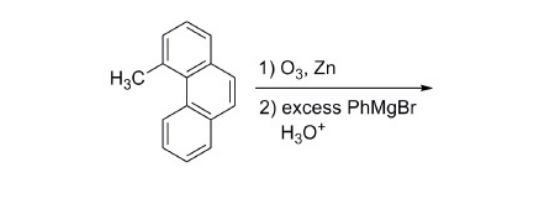
\includegraphics[width=0.35\textwidth]{figs/image12.png}
\caption{Structure for stereoisomeric product question}
\label{fig:q56}
\end{figure}

\hfill{\brak{\textbf{GATE CY 2015}}}

\textcolor{green}{\textbf{Correct Answer :}} 8


%----------------- Q57 ------------------
\item 
The major product formed in the following reaction is 
\begin{figure}[H]
\centering
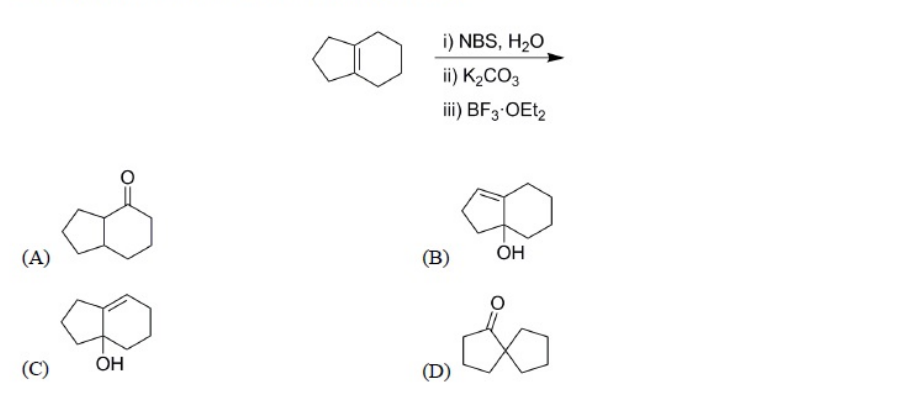
\includegraphics[width=\textwidth]{figs/image13.png}
\caption{Reaction with NBS, H$_2$O, K$_2$CO$_3$, BF$_3$.OEt$_2$}
\label{fig:q57}
\end{figure}



\hfill{\brak{\textbf{GATE CY 2015}}}

\begin{multicols}{2}
\begin{enumerate}[leftmargin=*, align=left]
    \item \wrong A
    \item \wrong B
    \item \wrong C
    \item \correct D
\end{enumerate}
\end{multicols}


%----------------- Q58 ------------------
\item 
The most suitable reagent(s) to effect the following transformation is
\begin{figure}[H]
\centering
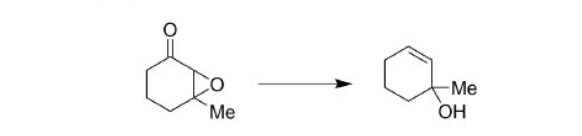
\includegraphics[width=0.7\textwidth]{figs/image14.png}
\caption{Reduction and transformation of cyclic ketone}
\label{fig:q58}
\end{figure}

\begin{enumerate}
    \item N$_2$H$_4$, KOH, heat
    \item TsNHNH$_2$, CF$_3$COOH
    \item LiAlH$_4$
    \item Na, liq. NH$_3$
\end{enumerate}

\hfill{\brak{\textbf{GATE CY 2015}}}

\begin{multicols}{2}
\begin{enumerate}[leftmargin=*, align=left]
    \item \wrong A
    \item \wrong B
    \item \wrong C
    \item \correct D
\end{enumerate}
\end{multicols}




%----------------- Q59 ------------------
\item 
The major product formed in the following reaction is
\begin{figure}[H]
\centering
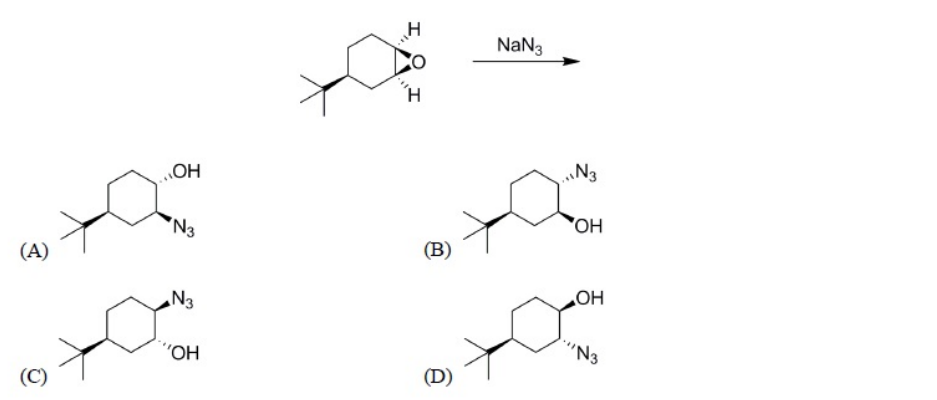
\includegraphics[width=\textwidth]{figs/image15.png}
\caption{Reaction of cyclohexane derivative with NaN$_3$}
\label{fig:q59}
\end{figure}

\begin{multicols}{2}
\begin{enumerate}[leftmargin=*, align=left]
\item \wrong A
\item \wrong B
\item \wrong C
\item \correct D
\end{enumerate}
\end{multicols}





%----------------- Q60 ------------------
\item 
Solvolysis of the optically active compound \textbf{X} gives, mainly
\begin{figure}[H]
\centering
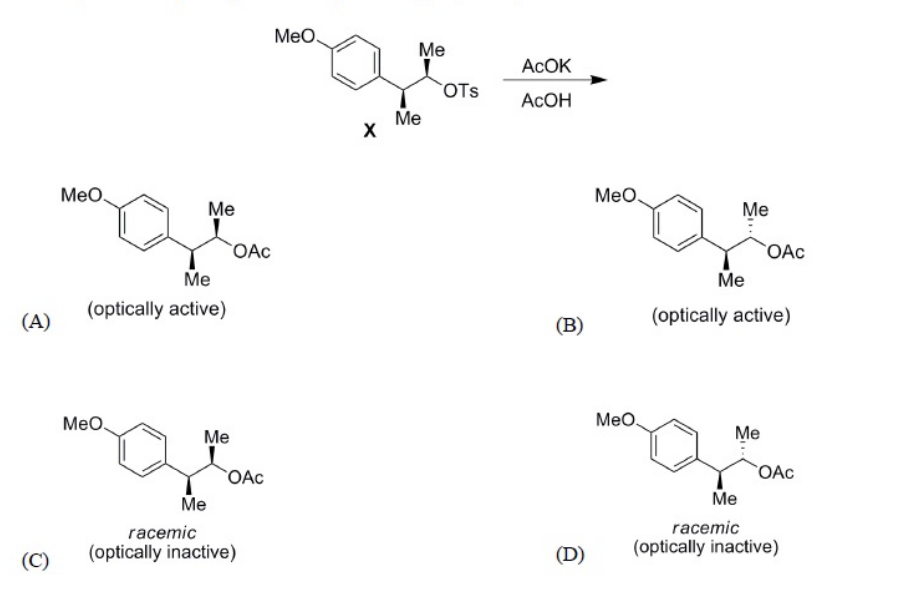
\includegraphics[width=\textwidth]{figs/image16.png}
\caption{Solvolysis reaction of optically active compound X}
\label{fig:q60}
\end{figure}

\begin{multicols}{2}
\begin{enumerate}[leftmargin=*, align=left]
\item \wrong A
\item \wrong B
\item \correct C
\item \wrong D
\end{enumerate}
\end{multicols}



%----------------- Q61 ------------------
\item 
The major product formed in the following reaction is
\begin{figure}[H]
\centering
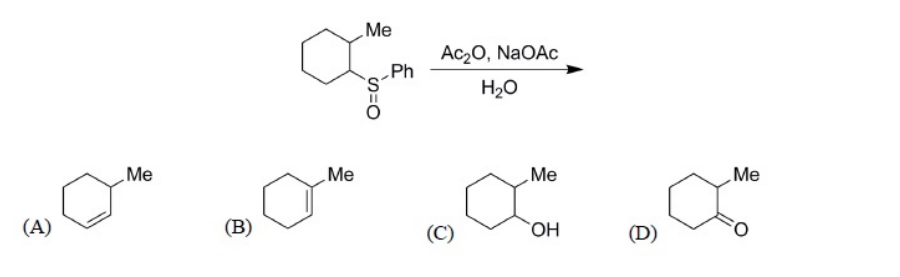
\includegraphics[width=\textwidth]{figs/image17.png}
\caption{Reaction showing formation of major product}
\label{fig:q61}
\end{figure}

\begin{multicols}{2}
\begin{enumerate}[leftmargin=*, align=left]
\item \wrong A
\item \wrong B
\item \wrong C
\item \correct D
\end{enumerate}
\end{multicols}

%----------------- Q62 ------------------
\item 
The tetrapeptide, Ala-Val-Phe-Met, on reaction with Sanger's reagent, followed by hydrolysis gives
\begin{figure}[H]
\centering
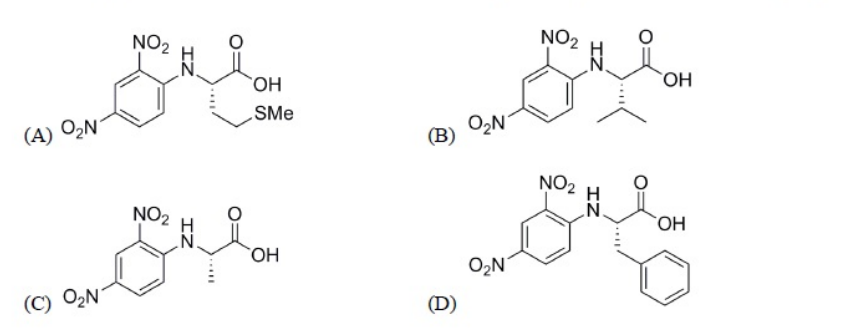
\includegraphics[width=\textwidth]{figs/image18.png}
\caption{Tetrapeptide reaction with Sanger's reagent and hydrolysis}
\label{fig:q62}
\end{figure}

\begin{multicols}{2}
\begin{enumerate}[leftmargin=*, align=left]
\item \wrong A
\item \wrong B
\item \correct C
\item \wrong D
\end{enumerate}
\end{multicols}



%----------------- Q63 ------------------
\item 
The major product formed in the following reaction is
\begin{figure}[H]
\centering
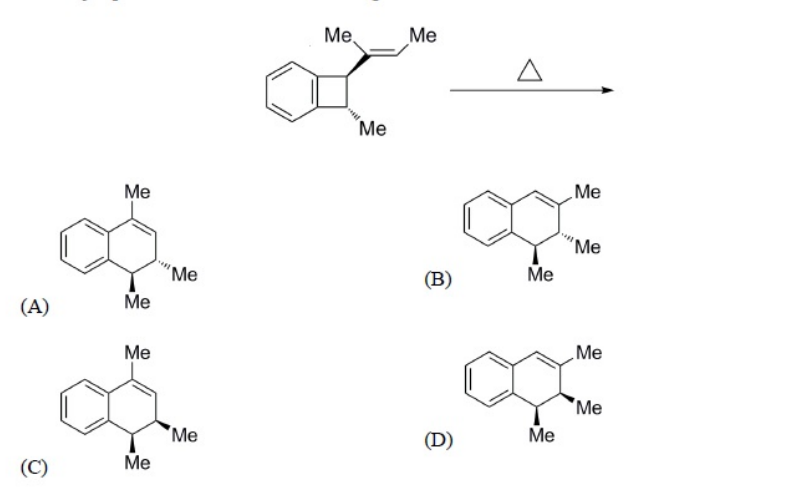
\includegraphics[width=0.7\textwidth]{figs/image19.png}
\caption{Reaction showing formation of major product}
\label{fig:q63}
\end{figure}

\begin{multicols}{2}
\begin{enumerate}[leftmargin=*, align=left]
\item \wrong A
\item \correct B
\item \wrong C
\item \wrong D
\end{enumerate}
\end{multicols}






%----------------- Q64 ------------------
\item 
The Beckmann rearrangement of a bromoacetophenone oxime (C$_8$H$_8$BrNO) gives a major product having the following $^1$H NMR ($\delta$, ppm): 9.89 (s, 1H), 7.88 (s, 1H), 7.45 (d, 1H, $J = 7.2$ Hz), 7.17 (m, 1H), 7.12 (d, 1H, $J = 7.0$ Hz), 2.06 (s, 3H). The structure of the product is
\begin{figure}[H]
\centering
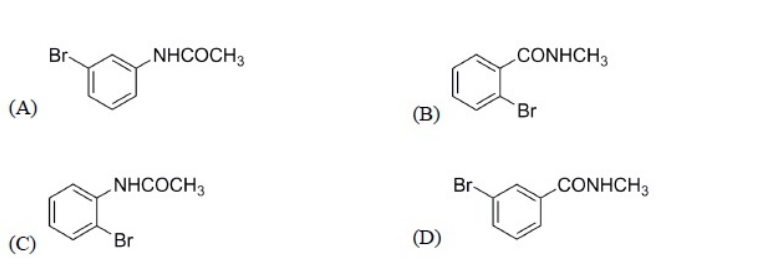
\includegraphics[width=\textwidth]{figs/image20.png}
\caption{Beckmann rearrangement product}
\label{fig:q64}
\end{figure}

\begin{multicols}{2}
\begin{enumerate}[leftmargin=*, align=left]
\item \correct A
\item \wrong B
\item \wrong C
\item \wrong D
\end{enumerate}
\end{multicols}





%----------------- Q65 ------------------
\item 
The major products, \textbf{K} and \textbf{L} formed in the following reactions are
\begin{figure}[H]
\centering
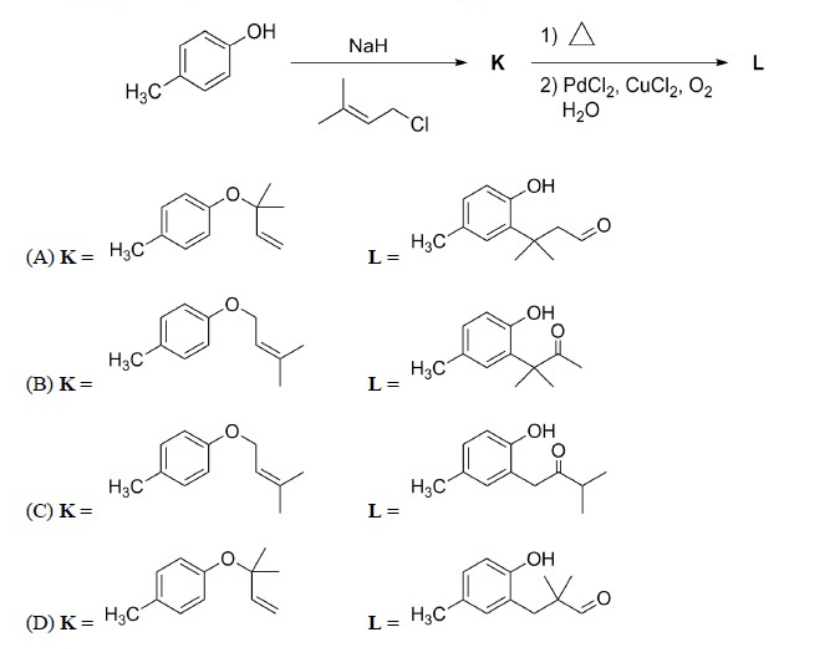
\includegraphics[width=0.8\textwidth]{figs/image21.png}
\caption{Major products K and L}
\label{fig:q65}
\end{figure}

\begin{multicols}{2}
\begin{enumerate}[leftmargin=*, align=left]
\item \wrong A
\item \correct B
\item \wrong C
\item \wrong D
\end{enumerate}
\end{multicols}

\end{enumerate}



\begin{center}
    \textbf{END OF THE QUESTION PAPER}
\end{center}





\end{document}

